\documentclass[a4paper]{report}

\usepackage{fontspec}
\usepackage{amssymb}
\usepackage{xltxtra}
\usepackage[lithuanian]{babel}
\usepackage{indentfirst}
\usepackage[]{hyperref}
\usepackage[]{amsmath}
\usepackage{amsthm}
\usepackage{amsfonts}
\usepackage{mathtools}
\usepackage{alltt}
%\usepackage{listingsutf8}

\hypersetup{pdfborder={0 0 0 0}}

\defaultfontfeatures{Mapping=tex-text}

% Aibių žymėjimai.
\newcommand\RSET{\mathop{\mathbb{R}}}
\newcommand\NSET{\mathop{\mathbb{N}}}

% tg, ctg, sign
\newcommand\tg{\mathop{\text{tg}}}
\newcommand\ctg{\mathop{\text{ctg}}}
\newcommand\sign{\mathop{\text{sign}}}

% Apibrėžimai, teiginiai, pastabos.
\swapnumbers

\theoremstyle{plain}
\newtheorem{prop}{Tg}

\theoremstyle{definition}
\newtheorem{defn}{Ap.}
\newtheorem{exmp}{Pvz}

\theoremstyle{remark}
\newtheorem*{note}{Pastaba}

\newtheoremstyle{notation}{3pt}{3pt}{}{}{\itshape}{:}{.5em}{}
\theoremstyle{notation}
\newtheorem*{notation}{Žymėjimas}

\title{%
Almanto Juozulyno\\
Matematinės analizės paskaitų konspektas}

\author{}
\date{\today}

\begin{document}

\maketitle
\bigskip
\tableofcontents
\chapter{Įžanga}

Čia turėtų būti kažkoks prasmingas tekstas.

\begin{defn}[Apibrėžimo pavyzdys]
  Čia turėtų būti apibrėžimas.
\end{defn}

\begin{exmp}[Pavyzdys]
  Čia turėtų būti pavyzdys.
\end{exmp}

\begin{note}
  Pastabos pavyzdys.
\end{note}

\begin{prop}
  Teiginio pavyzdys.
  \begin{proof}
    Teiginio įrodymas.
  \end{proof}
\end{prop}
                 % Įžanginė.
\chapter{Funkcijos riba}

\begin{notation}
  Funkcija iš realiųjų skaičių aibės $A$ į visų realiųjų skaičių aibę 
  $\RSET$ žymima:
  \[
  \begin{array}[]{c l}
    f : A \to \RSET, & \text{kur $A$ – funkcijos $f$ apibrėžimo sritis.}
  \end{array}
  \]
\end{notation}

\begin{defn}[$\varepsilon$-aplinka]
  \[
  B(\varepsilon; a) = U(\varepsilon; a) =%
  \{ x \in \RSET : |x - a| < \varepsilon \}
  \]
\end{defn}

\begin{defn}[Taško aplinka]
  Taško $a$ aplinka vadinsime aibę $A$, kuriai:
  \[
  \varepsilon > 0 : \exists U(\varepsilon; a) \subset A
  \]
\end{defn}

\begin{defn}[Atvira aibė]
  Aibė $A$ vadinama atvira aibe, jei ji yra kiekvieno savo taško aplinka.
\end{defn}

\begin{defn}[Uždara aibė]
  Aibė $A$ vadinama uždara aibe, jei $\RSET \setminus A$ yra atvira aibė.
\end{defn}

\begin{note}
  Jei taškas $a \in \{-\infty; +\infty\}$, tai jo aplinka:
  \begin{align*}
    U(\varepsilon; +\infty) &= (\varepsilon; +\infty) \\
    U(\varepsilon; -\infty) &= (-\infty; -\varepsilon)
  \end{align*}
\end{note}

\begin{notation}
  Taško $a (a \in \RSET \cup \{-\infty;+\infty\})$ aplinka žymima:
  $U_{a}$ arba $V_{a}$.
\end{notation}

Šiuose apibrėžimuose laikome, jog $A \subset \RSET$:
\begin{enumerate}
  \item 
    \begin{defn}[Aibės ribinis taškas]
      Taškas $a (a \in \RSET)$ vadinamas aibės $A$ ribiniu tašku, jei 
      $\forall \varepsilon (\varepsilon > 0)$ egzistuoja bent du aibės
      taškai priklausantys $U(\varepsilon; a)$.
    \end{defn}
  \item
    \begin{defn}[Aibės vidinis taškas]
      Taškas $a (a \in \RSET)$ vadinamas vidiniu aibės $A$ tašku, jei 
      $\exists \varepsilon (\varepsilon > 0)$, kad 
      $U(\varepsilon; a) \subset A$.
    \end{defn}
  \item 
    \begin{defn}[Aibės sienos taškas]
      Taškas $a (a \in \RSET)$ vadinamas aibės $A$ sienos tašku, jei 
      $\forall \varepsilon (\varepsilon > 0)$ 
      $U(\varepsilon; a)$ turės tašką iš aibės $A$ ir tašką 
      nepriklausantį $A$.
    \end{defn}
  \item 
    \begin{defn}[Aibės izoliuotas taškas]
      Taškas $a (a \in \RSET)$ vadinamas aibės $A$ izoliuotu tašku, jei
      $a \in A$ ir $\exists \varepsilon (\varepsilon > 0)$, 
      $U(\varepsilon; a)$, kurioje be $a$ nėra kitų aibės taškų.
    \end{defn}
\end{enumerate}
                 % Funkcijos riba.
\begin{prop}
  Jei $\lim_{x \to a} f(x) = b$ ir $\lim_{x \to a} f(x) = c$, tai $b = c$.
  \begin{proof}
    Tarkime priešinai $b \neq c$. Tegu $b < c$.

    Pagal \ref{limfed} apibrėžimą:
    \begin{align*}
      \lim_{x \to a} f(x) = b \iff&% 
        \forall U_{b}, \exists U_{a} :%
        f(x) \in U_{b}, \forall x(x \in U_{a}) \\
      \lim_{x \to a} f(x) = c \iff&% 
        \forall U_{c}, \exists U'_{a} :%
        f(x) \in U_{c}, \forall x(x \in U'_{a})
    \end{align*}

    Pastebėkime, kad $U_{a} \cap U'_{a}$ bus taško $a$ aplinka (taško 
    aplinka visada yra netuščia aibė).
    Fiksuojame tokias $U_{b}$ ir $U_{c}$, kurioms 
    $U_{b} \cap U_{c} = \emptyset$. Bet 
    $\forall x (x \in U_{a} \cap U'_{a}) \implies% 
      f(x) \in U_{b} \land f(x) \in U_{c}$, gavome prieštarą.
  \end{proof}
\end{prop}

\begin{prop}
  Jei $f(x) \leq g(x), \forall x (x \in U_{a})$ ir $f$ bei $g$ turi ribą
  taške $a$, tai $\lim_{x \to a} f(x) \leq \lim_{x \to a} g(x)$.
  %TODO: Įrodyti!
\end{prop}

\begin{prop}
  Jei $\lim_{x \to a} f(x) = b < c$, tai 
  $\exists U_{a} : f(x) < c, \forall x (x \in U_{a})$.
  %TODO: Įrodyti!
\end{prop}

\begin{prop}
  Jei $h(x) \leq f(x) \leq g(x), \forall x(x \in A)$ ir 
  $\lim_{x \to a} h(x) = \lim_{x \to a} g(x) = b$, tai
  $\lim_{x \to a} f(x) = b$.
  %TODO: Įrodyti!
\end{prop}

\begin{prop}
  Jei $f$ yra monotoniška intervale $I$ ir $a \in I$, tai 
  $\exists \lim_{x \to a} f(x)$. Jei papildomai žinome, kad $f$ yra
  aprėžta intervale $I$, tai $\lim_{x \to a} f(x)$ yra baigtinė.
  %TODO: Įrodyti!
\end{prop}

\begin{prop}
  Jei $f$ ir $g$ turi baigtines ribas taške $a$ ir 
  $\alpha, \beta \in \RSET$, tai 
  \begin{enumerate}
    \item \[
      \lim_{x \to a} (\alpha f(x) + \beta g(x)) =%
        \alpha \lim_{x \to a} f(x) + \beta \lim_{x \to a} g(x);
      \]
    \item \[
      \lim_{x \to a} (f(x)g(x)) =%
        \lim_{x \to a} f(x) \lim_{x \to a} g(x);
      \]
    \item Jei 
      $g(x) \neq 0, \forall x (x \in A), \lim_{x \to a} g(x) \neq 0$, tai
      \begin{equation*}
        \lim_{x \to a} \frac{f(x)}{g(x)} =
          \frac{\lim_{x \to a} f(x)}{\lim_{x \to a} g(x)}.
      \end{equation*}
  %TODO: Įrodyti!
  \end{enumerate}
\end{prop}

\begin{defn}[Funkcijos riba iš dešinės]
  Taškas $b$ vadinamas funkcijos $f$ riba taške $a$ iš dešinės, jei:
  \[
  \forall U_{b}, \exists U_{a} :%
    f(x) \in U_{b}, \forall x (x \in U_{a} \cap (a; +\infty)).
  \]
  \begin{notation} 
    \[
    \lim_{x \to a^{+}} f(x) = b
    \]
  \end{notation}
\end{defn}

\begin{defn}[Funkcijos riba iš kairės]
  Taškas $b$ vadinamas funkcijos $f$ riba taške $a$ iš kairės, jei:
  \[
  \forall U_{b}, \exists U_{a} :%
    f(x) \in U_{b}, \forall x (x \in U_{a} \cap (-\infty; a)).
  \]
  \begin{notation} 
    \[
    \lim_{x \to a^{-}} f(x) = b
    \]
  \end{notation}
\end{defn}

TODO: Įkelti per praktiką darytus pavyzdžius.
                 % Funkcijos riba.
\section{Koši kriterijus}

\begin{note}
  Toliau tekste daroma prielaida, jog $f: A \to \RSET$ ir $a$ yra 
  aibės $A$ ribinis taškas.
\end{note}

\begin{prop}
  (Koši kriterijus) Funkcija $f$ turi baigtinę ribą taške $a$
  (taškas $a$ gali būti ir $\infty$) tada ir tik tada:
  \begin{equation}
    \forall \varepsilon (\varepsilon > 0), \exists U_{a} :
    | f(x') - f(x'') | < \varepsilon,
    \forall x', x'' (x',x'' \in U_{a} \cap A, x' \neq a, x'' \neq a)
    \label{kosi}
  \end{equation}

  \begin{proof}
    \hfill \\
    \begin{description}
      \item[Būtinumas] Tarkime, jog $\exists \lim_{x \to a} f(x)$ ir ji
        yra baigtinė. Reikia įrodyti \ref{kosi} teiginį.

        Pažymėkime:
        \begin{equation*}
          \lim_{x \to a} f(x) = b.
        \end{equation*}

        Tada pagal funkcijos ribos apibrėžimą (\ref{limfed}):
        \begin{equation*}
          \lim_{x \to a} f(x) = b \iff 
          \forall \varepsilon (\varepsilon > 0), \exists U_{a}:
          | f(x) - b | < \varepsilon, 
          \forall x (x \in U_{a} \cap A \setminus \{a\}).
        \end{equation*}

        Tada galime įvertinti:
        \begin{align*}
          | f(x') - f(x'') | &= | f(x') - b + b - f(x'') | \\
          &\leq \underbrace{| f(x') - b |}_{ < \varepsilon } +
          \underbrace{| f(x'') - b |}_{ < \varepsilon } \\
          &< 2 \varepsilon, \forall x',x'' 
          (x',x'' \in U_{a} \cap A \setminus \{a\}).
        \end{align*}

      \item[Pakankamumas] Tarkime, kad \ref{kosi} sąlyga teisinga. Reikia 
        įrodyti, kad $\exists \lim_{x \to a} f(x)$ ir kad ji yra baigtinė.

        Kadangi \ref{kosi} teisinga, tai:
        \begin{equation}
          \forall \varepsilon (\varepsilon > 0), \exists U_{a} :
          | f(x') - f(x'') | < \varepsilon, \forall x',x''
          (x',x'' \in U_{a} \cup A \setminus \{a\})
          \label{_kosi_01}
        \end{equation}

        Imame bet kokią seką $\left\{ x_{n} \right\}, x_{n} \to a$. Pagal
        sekos ribos apibrėžimą:
        \begin{equation}
          \forall U_{a}, \exists N (N \in \NSET) : 
            x_{n} \in U_{a}, \forall n (n > N)
          \label{_kosi_02}
        \end{equation}

        Tada iš \ref{_kosi_01} ir \ref{_kosi_02} gauname:
        \begin{equation}
          | f(x_{n}) - f(x_{m}) | < \varepsilon : \forall n, m (n,m > N)
          \label{_kosi_03}
        \end{equation}

        Iš Koši kriterijaus skaičių sekoms ir \ref{_kosi_03} gauname, kad
        seka $\left\{ f(x_{n}) \right\}$ turi baigtinę ribą.

        Tam, kad pilnai būtų patenkintas \ref{limfs} funkcijos ribos 
        apibrėžimas, reikia, kad ir 
        $\left\{ x'_{n} \right\}, x'_{n} \to a : \left\{ f(x'_{n}) \right\}$
        turėtų tą pačią ribą, kaip ir $\left\{ f(x_{n}) \right\}$, 
        kai $x_{n} \to a$.

        Sukonstruokime seką
        \begin{equation*}
          x_{1},x'_{1},x_{2},x'_{2},x_{3},x'_{3},\ldots
        \end{equation*}
        ir pažymėkime ją $\left\{ y_{n} \right\}$.

        Kadangi sekos $\left\{ y_{n} \right\}$ posekiai 
        $\left\{ x_{n} \right\}$ ir $\left\{ x'_{n} \right\}$, kurie pilnai 
        padengia visus jos narius, artėja į $a$, tai ir seka 
        $\left\{ y_{n} \right\}$ artėja į $a$.

        Iš Koši kriterijaus skaičių sekoms gauname, jog 
        $\left\{ f(y_{n}) \right\}$ turi baigtinę ribą. Iš skaičių sekos
        ribos apibrėžimo neprieštaringumo gauname, jog 
        $\left\{ f(y_{2n}) \right\} = \left\{ f(x'_{n}) \right\}$ ir
        $\left\{ f(y_{2n+1}) \right\} = \left\{ f(x_{n}) \right\}$ turi tą
        pačią ribą.

    \end{description}
  \end{proof}
\end{prop}

\section{Ribų skaičiavimo pavyzdžiai}

\begin{exmp}
  \label{lim_sinx_x}
  Įrodysime, kad:
  \begin{equation*}
    \lim_{x \to 0} \frac{\sin x}{x} = 1
  \end{equation*}

  \begin{proof}

    Nubrėžkime vienetinį apskritimą ($|OD| = |OB| = 1$). Iš 
    brėžinio (\ref{fig:sinx_x}) matome, jog:
    \begin{equation}
      S _{\triangle OBD} \leq S _{\text{išp.}OBD} \leq S _{\triangle OBC}
      \label{_sinx_x_01}
    \end{equation}

    \begin{figure}[h!]
      \begin{center}
        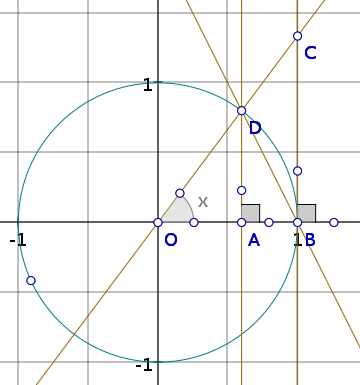
\includegraphics[]{images/sinx_x.png}
      \end{center}
      \caption{Brėžinys.}
      \label{fig:sinx_x}
    \end{figure}

    Apskaičiuokime trikampio $ODB$ plotą:
    \begin{align*}
      S _{\triangle OBD} &= \frac{ |AD| |OB| }{2} \\
      &= \frac{ |AD| }{2}, &\left\{ \text{ nes } |OB| = 1 \right\} \\
      &= \frac{ |OD| \sin x }{2}, 
      &\left\{ \text{ nes } \frac{ |AD| }{ |OD| } = \sin x \right\} \\
      &= \frac{ \sin x }{2}, &\left\{ \text{ nes } |OD| = 1 \right\}.
    \end{align*}

    Skritulio plotas lygus:
    \begin{equation*}
      S = \pi |OD|^2
    \end{equation*}

    Išpjovos $S_{\text{išp.}OBD}$ plotas sudaro $\frac{x}{2 \pi}$ viso 
    skritulio ploto:
    \begin{align*}
      S_{\text{išp.}OBD} &= S \frac{x}{2 \pi} \\
      &= \frac{\pi |OD|^2 x}{2 \pi} \\
      &= \frac{x}{2}
    \end{align*}

    Apskaičiuokime trikampio $OBC$ plotą:
    \begin{align*}
      S_{\triangle OBC} &= \frac{ |OB| |BC| }{2} \\
      &= \frac{ |OB| (|OB| \tg x)}{2}, 
        &\left\{ \text{ nes } \frac{|BC|}{|OB} = \tg x \right\} \\
      &= \frac{\tg x}{2} &\left\{ \text{ nes } |OB| = 1 \right\}
    \end{align*}

    Įsistatę išraiškas į \ref{_sinx_x_01} gauname:
    \begin{equation*}
      \frac{\sin x}{2} \leq \frac{x}{2} \leq \frac{\tg x}{2}
    \end{equation*}

    Pertvarkę gauname:
    \begin{align}
      \sin x \leq x & \text{ ir } \label{_sinx_x_02} \\
      x \leq \tg x. \label{_sinx_x_03}
    \end{align}

    Iš \ref{_sinx_x_02} gauname:
    \begin{equation}
      \frac{\sin x}{x} \leq 1 
      \label{_sinx_x_04}
    \end{equation}

    O iš \ref{_sinx_x_03}:
    \begin{align}
      x & \leq \tg x = \frac{\sin x}{\cos x} \\
      \cos x &\leq \frac{\sin x}{x}.
      \label{_sinx_x_05}
    \end{align}

    Iš \ref{_sinx_x_04} ir \ref{_sinx_x_05}:
    \begin{align}
      \cos x &\leq \frac{\sin x}{x} \leq 1 \\
      \cos x - 1 &\leq \frac{\sin x}{x} - 1 \leq 0 \\
      0 &\leq 1 - \frac{\sin x}{x} \leq 1 - \cos x
    \end{align}

    Pasinaudodami \ref{f_tri_kvsum} ir \ref{f_tri_dkcos} trigonometrinėmis
    tapatybėmis $1 - \cos x$ galime pertvarkyti:
    \begin{align}
      1 - \cos x &= \left( \cos^2 \frac{x}{2} + \sin^2 \frac{x}{2} \right) 
        - \left( \cos^2 \frac{x}{2} - \sin^2 \frac{x}{2} \right) \\
      &= 2 \sin^2 \frac{x}{2} \\
      &\leq 2 \left( \frac{x}{2} \right)^2 
        &\left\{ \text{Pasinaudojame \ref{_sinx_x_02} neligybe.} \right\} \\
      &= \frac{x^2}{2}.
    \end{align}

    Pagal trijų girtuoklių teoremą, kadangi:
    \begin{align*}
      \lim_{x \to 0^{+}} 0 &= 0 &\text{ ir } \\
      \lim_{x \to 0^{+}} \frac{x^2}{2} &= 0 &\text{ tai ir } \\
      \lim_{x \to 0^{+}} \left( 1 - \frac{\sin x}{x} \right) &= 0, 
        &\text{o tai reiškia, kad} \\
      \lim_{x \to 0^{+}} \frac{\sin x}{x} &= 1.
    \end{align*}

    Pažymėję $y = -x$, gauname:
    \begin{align*}
      \lim_{x \to 0^{-}} \frac{\sin x}{x} &=
      \lim_{x \to 0^{-}} \frac{-\sin x}{-x} \\
      &= \lim_{x \to 0^{-}} \frac{\sin(-x)}{-x} \\
      &= \lim_{y \to 0^{+}} \frac{\sin y}{y} = 1
    \end{align*}

    Kadangi egzistuoja riba iš dešinės ir iš kairės, ir jos sutampa, tai
    \begin{equation*}
      \lim_{x \to 0} \frac{\sin x}{x} = 1
    \end{equation*}

  \end{proof}

\end{exmp}

\begin{exmp}
  Įrodysime, kad:
  \begin{equation}
    \lim_{x \to 0} (1 + x)^{\frac{1}{x}} = e
    \label{_fx_e_01}
  \end{equation}

  \begin{proof}

    Iš pradžių įrodysime, kad funkcijos $f(x) = (1 + x)^{\frac{1}{x}}$ 
    riba iš dešinės taške $x = 0$ yra lygi $e$.

    Sakykime, $x_k > 0$ ir $x_k \to 0 (k \in \NSET)$. Pažymėkime $n_k$ 
    mažiausią natūrinį skaičių, didesnį už $\frac{1}{x_k}$, tai yra 
    \begin{equation*}
      n_{k} = min \left\{ n \in \NSET : n > \frac{1}{x_{k}} \right\}
    \end{equation*}
    Iš Archimedo principo žinome, kad toks skaičius visada egzistuoja.
    Dabar galime įvertinti $\frac{1}{x_k}$:
    \begin{equation*}
      n_k - 1 \leq \frac{1}{x_k} < n_k.
    \end{equation*}

    Atlikę trivialius pertvarkymus gauname $x_k$ įvertinimą:
    \begin{equation*}
      \frac{1}{n_{k}} < x_k \leq \frac{1}{n_{k} - 1}.
    \end{equation*}

    Akivaizdu, kad $(1 + x_{k})^\frac{1}{x_{k}}$ pagrindą ir laipsnį 
    pakeitę ne didesniais, gausime ne didesnį skaičių. Tai yra:
    \begin{equation}
      \left( 1 + \frac{1}{n_{k}} \right)^{n_{k} - 1}
      \leq (1 + x_{k})^\frac{1}{x_{k}}.
      \label{_fx_e_03}
    \end{equation}

    Taip pat pakeitę ne mažesniais gausime ne mažesnį skaičių:
    \begin{equation}
      (1 + x_{k})^{\frac{1}{x_{k}}} 
      \leq \left( 1 + \frac{1}{n_{k} - 1} \right)^{n_{k}}
      \label{_fx_e_04}
    \end{equation}

    Kairiąją \ref{_fx_e_03} nelygybės pusę galime pertvarkyti į 
    \begin{equation}
      \underbrace{\left( 1 + \frac{1}{n_{k}} \right)^{-1}}_{\to 1}
      \underbrace{\left( 1 + \frac{1}{n_{k}} \right)^{n_{k}}}_{\to e}
      \label{_fx_e_05}
    \end{equation}

    Dešiniąją \ref{_fx_e_04} nelygybės pusę galime pertvarkyti į
    \begin{equation}
      \underbrace{\left( 1 + \frac{1}{n_{k}-1} \right)^{n_{k}-1}}_{\to e}
      \underbrace{\left( 1 + \frac{1}{n_{k}-1} \right)^{1}}_{\to 1}
      \label{_fx_e_06}
    \end{equation}

    Kadangi skaičių $y_{n} = (1 + \frac{1}{n})^n$ seka, kai 
    $n \to +\infty$, turi ribą $e$, tai ir seka $y_{n_{k}}$, kuri
    gali skirtis nuo sekos $y_{n}$ posekio tik narių tvarka turi 
    tą pačią ribą $e$. Taigi \ref{_fx_e_05} ir \ref{_fx_e_06} 
    konverguoja į skaičių $e$. Todėl, pagal dviejų policininkų
    principą, ir seka $(1 + x_{k})^{\frac{1}{x_{k}}}$ konverguoja į
    $e$. Pagal funkcijos ribos apibrėžimą sekoms (\ref{limfs})
    gauname:
    \begin{equation}
      \lim_{x \to 0^{+}} (1 + x)^{\frac{1}{x}} = e.
      \label{_fx_e_07}
    \end{equation}

    Dabar įrodysime, kad ir 
    $\lim_{x \to 0^{-}} (1 + x)^{\frac{1}{x}} = e$. Sakykime, kad
    $-1 < x < 0$ ir pažymėkime $y = -x$. Tada
    \begin{align*}
      \lim_{x \to 0^{-}} (1 + x)^{\frac{1}{x}} 
      &= \lim_{y \to 0^{+}} (1 - y)^{-\frac{1}{y}} \\
      &= \lim_{y \to 0^{+}} 
        \left( \frac{1}{1 - y} \right)^{\frac{1}{y}} \\
      &= \lim_{y \to 0^{+}} 
        \left( 1 + \frac{1}{1 - y} - 1 \right)^{\frac{1}{y}} \\
      &= \lim_{y \to 0^{+}} 
        \left( 1 + \frac{y}{1 - y} \right)^{\frac{1}{y}} \\
      &= \lim_{y \to 0^{+}} 
        \left( 1 + \frac{y}{1 - y} \right)^{\frac{1}{y} - 1}
        \left( 1 + \frac{y}{1 - y} \right)^{1} \\
      &= \lim_{y \to 0^{+}} 
        \underbrace{
          \left( 1 + \frac{y}{1 - y} \right)^{\frac{1 - y}{y}}}_{\to e}
        \underbrace{
          \left( 1 + \frac{y}{1 - y} \right)^{1}}_{\to 1} \\
      &= e.
    \end{align*}

  \end{proof}
\end{exmp}
                 % Funkcijos riba.
\section{Viršutinė ir apatinė ribos}

\begin{defn}[Viršutinė riba]
  \begin{equation*}
    \limsup _{x \to a} f(x) := 
      \lim _{\delta \to 0} 
      \sup \left\{ f(x), x \in A : |x - a| < \delta \right\}
  \end{equation*}
\end{defn}

\begin{defn}[Apatinė riba]
  \begin{equation*}
    \liminf _{x \to a} f(x) :=
      \lim _{\delta \to 0}
      \inf \left\{ f(x), x \in A : |x - a| < \delta \right\}
  \end{equation*}
\end{defn}

\begin{exmp}
  \begin{align*}
    \limsup _{x \to 0} \left( \sin \frac{1}{x} \right) 
    &= \lim _{\delta \to 0} \sup 
      \left\{ \sin \frac{1}{x} : |x - a| < \delta \right\} \\
    &= \lim _{\delta \to 0} 1 \\
    &= 1
  \end{align*}
  \begin{align*}
    \liminf _{x \to 0} \left( \sin \frac{1}{x} \right) 
    &= \lim _{\delta \to 0} (-1) = -1
  \end{align*}
\end{exmp}

\begin{prop}
  \begin{equation*}
    \exists \lim _{x \to a} f(x) \iff
    \limsup _{x \to a} f(x) = \liminf _{x \to a} f(x)
  \end{equation*}
\end{prop}

\begin{defn}[Viršutinė riba]
  \begin{equation*}
    \limsup _{x \to a} f(x) :=
      \lim _{\delta \to 0}
      \sup \left\{ f(x) : x 
        (x \in U(a, \delta) \cap A \setminus \{a\}) 
        \right\}
  \end{equation*}
\end{defn}

\begin{defn}[Apatinė riba]
  \begin{equation*}
    \liminf _{x \to a} f(x) :=
      \lim _{\delta \to 0}
      \inf \left\{ f(x) : x 
        (x \in U(a, \delta) \cap A \setminus \{a\}) 
        \right\}
  \end{equation*}
\end{defn}

\begin{notation}
  \begin{align*}
    \lim _{x \to a^{+}} f(x) &\equiv f(a^{+}) \\
    \lim _{x \to a^{-}} f(x) &\equiv f(a^{-}) \\
  \end{align*}
\end{notation}

TODO: Įkelti pavyzdį.

\section{Monotoniškos funkcijos}

\begin{prop}
  \label{lim_mon}
  $f: A \to \RSET$, $a$ – ribinis ir didžiausias $A$ taškas ir $f$ yra
  monotoniška. Tada $f$ turi ribą taške $a$. Ir jei $f$ yra ir apibrėžta,
  tai riba taške $a$ yra baigtinė.
\end{prop}

\begin{exmp}
  Įrodyti, kad $f(x), f(x) = x^2$, taške $a, a = 1$, turi baigtinę ribą.
  Apibrėžimo sritis $A = \left( \frac{1}{2}; 1 \right)$.

  \begin{proof}
    Pirma parodysime, kad $f(x)$ intervale $A$ didėja. Paimkime 
    $x_{1}$ ir $x_{2}$, tokius, kad $x_{1} < x_{2}$. Tada:

    \begin{align*}
      f(x_{2}) - f(x_{1}) 
      &= x _{2} ^{2} - x _{1} ^{2} \\
      &= \underbrace{(x_{2} - x_{1})}_{> 0}
        \underbrace{(x_{2} + x_{1})}_{> 0}
    \end{align*}

    Gavome, kad $f(x_{2}) > f(x_{1})$, o tai reiškia, kad $f(x)$ intervale
    $\left( \frac{1}{2} ; 1 \right)$ didėja. Taigi pagal \ref{lim_mon}
    teiginį $\exists \lim _{x \to a} f(x)$.

    Ar $f(x)$ yra aprėžta? Tai yra ar
    \begin{equation*}
      \exists c (c \in \RSET) : x^{2} \leq c, \forall x (x \in A)?
    \end{equation*}
    Taip $c = 1$. Taigi $\lim _{x \to 1} x^{2}$ yra baigtinė.
  \end{proof}
\end{exmp}

\section{Funkcijos tolydumas}

\begin{defn}[Tolydi taške funkcija]
  Funkcija $f$ vadiname tolydžia taške $a$, jei 
  \begin{equation*}
    \forall U_{f(a)}, \exists U_{a} : 
      f(x) \in U_{f(a)}, \forall x (x \in U_{a} \cap A)
  \end{equation*}
\end{defn}

$f(x)$ gali būti tolydi taške $a$ dviem atvejais:
\begin{enumerate}
  \item jei $a$ – izoliuotas aibės $A$ taškas, ir 
  \item jei $a$ – ribinis aibės $A$ taškas bei 
    $\lim _{x \to a} f(x) = f(a)$.
\end{enumerate}

\begin{defn}[Tolydi aibėje funkcija]
  Funkcija $f$ vadinama tolydžia aibėje $B$, jei ji yra tolydi visuose
  aibės $B$ taškuose.
\end{defn}

\begin{note}
  Toliau $f: A \to B$ ir $a \in A$.
\end{note}

\begin{defn}[Trūkio taškų tipai]
  \begin{description}
    \hfill \\
    \item[1 rūšies trūkis] Jei 
      \begin{equation*}
        \exists \lim _{x \to a^{-}} f(x) 
        \text{ ir }
        \exists \lim _{x \to a^{+}} f(x) 
      \end{equation*}
       ir jos abi yra baigtinės, tai
      taškas a yra vadinamas 1 rūšies trūkiu.
    \item[pataisomas trūkis] Jei
      \begin{equation*}
        \lim _{x \to a^{-}} f(x) = \lim _{x \to a^{-}} f(x) 
        \implies \exists \lim _{x \to a} f(x)
      \end{equation*}
      yra baigtinė, tai taškas $a$ vadinamas pataisomu trūkio tašku.
    \item[2 rūšies trūkis] Jei
      \begin{equation*}
        \nexists \lim _{x \to a^{-}} f(x)
        \text{ arba }
        \nexists \lim _{x \to a^{+}} f(x),
      \end{equation*}
      arba bent viena iš jų yra begalinė, tai taškas $a$ yra vadinamas
      2 rūšies trūkiu.
  \end{description}
\end{defn}

\begin{exmp}
  \begin{equation*}
    f(x) = \frac{x}{x}, a = 0
  \end{equation*}

  Kadangi $\lim _{x \to 0} f(x) \neq f(0)$, nes $\nexists f(0)$, tai
  taškas $x = 0$ yra trūkio.

  Kadangi $\lim _{x \to 0} \frac{x}{x} = 1$, tai $x = 0$ yra 1 rūšies
  trūkio taškas ir jis yra pataisomas.
\end{exmp}

\begin{exmp}
  \begin{equation*}
    f(x) = \sign(x), a = 0
  \end{equation*}

  Kadangi
  \begin{align*}
    \lim _{x \to 0^{+}} \sign(x) &= 1 \\
    \lim _{x \to 0^{-}} \sign(x) &= -1,
  \end{align*}
  tai $x = 0$ yra 1 rūšies trūkio taškas.
\end{exmp}

\begin{exmp}
  \begin{equation*}
    f(x) = \frac{1}{|x|}, a = 0
  \end{equation*}

  Kadangi
  \begin{align*}
    \lim _{x \to 0^{+}} \frac{1}{|x|} &= +\infty \\
    \lim _{x \to 0^{-}} \frac{1}{|x|} &= +\infty,
  \end{align*}
  tai $x = 0$ yra 2 rūšies trūkio taškas.
\end{exmp}

\begin{prop}
  Jei $f$ ir $g$ yra tolydžios taške $a$, tai ir 
  $f + g$, $f - g$, $f \cdot g$ bei $\frac{f}{g}$ (jei $g(a) \neq 0$) 
  yra tolydžios taške $a$.

  \begin{proof}
    Žymėjimas:
    \begin{equation*}
      (f + g)(x) := f(x) + g(x)
    \end{equation*}

    Įrodysime, kad jei $f$ ir $g$ yra tolydžios taške $a$, tai ir 
    $(f + g)(x)$ yra tolydi taške $a$.

    Tarkime, jog $f$ ir $g$ yra tolydžios taške $a$. Reikia įrodyti:
    \begin{equation*}
      \lim _{x \to a} (f + g)(x) = (f + g)(a)
    \end{equation*}

    Tikriname:
    \begin{align*}
      \lim _{x \to a} (f + g)(x)
      &= \lim _{x \to a} (f(x) + g(x)) \\
      &= \lim _{x \to a} f(x) + \lim _{x \to a} g(x) \\
      &= f(a) + g(a)
      &= (f + g)(a)
    \end{align*}
  \end{proof}
\end{prop}

\begin{prop}
  $ (f \circ g)(x) := f(g(x))$ Jei $g$ yra tolydi taške $a$ ir 
  $f$ yra tolydi taške $g(a)$, tai $f \circ g$ yra tolydi taške $a$.
\end{prop}
                 % Funkcijos riba.
\begin{prop}
  (I Vejerštraso) Tolydi funkcija $f$ uždarame, aprėžtame intervale yra
  aprėžta. ($f : [a;b] \to \RSET$, kur $a, b \neq \infty$)

  \begin{proof}
    Tarkime $f$ nėra aprėžta iš viršaus. Iš priešingo apibrėžimo:
    \begin{equation*}
      \forall n (n \in \NSET), \exists x_{n} (x_{n} \in [a;b]) :
        f(x_{n}) > n
    \end{equation*}

    Sukonstravome seką $\left\{ x_{n} \right\}$, kur 
    $a \leq x_{n} \leq b$. Iš Vejerštraso teoremos skaičių sekoms:
    $ \exists x_{n_{k}}$, kur $x_{n_{k}} \to x'$, 
    kai $n_{k} \to +\infty$.

    Iš skaičių sekų ribų elementariųjų savybių, kadangi 
    $a \leq x_{n_{k}} \leq b$ ir $x_{n_{k}} \to x'$, tai 
    $a \leq x' \leq b$.

    Kadangi $f$ yra tolydi, tai 
    \begin{equation*}
      \lim _{x \to x'} f(x) = f(x'),
    \end{equation*}
    o tai reiškia, kad
    \begin{equation*}
      \lim _{x_{n_{k}} \to x'} f(x) = f(x') \neq +\infty.
    \end{equation*}

    Tuo tarpu iš to, kad
    \begin{equation*}
      \forall n (n \in \NSET), \exists x_{n} (x_{n} \in [a;b]) :
        f(x_{n}) > n
    \end{equation*}
    seka, jog
    \begin{equation*}
      \lim _{x_{n_{k}} \to x'} f(x_{n_{k}}) = +\infty.
    \end{equation*}

    Gavome prieštarą. Vadinasi $f$ yra aprėžta iš viršaus. 

    Analogiškai galime įrodyti, kad $f$ yra aprėžta iš apačios.
  \end{proof}

\end{prop}

\begin{exmp}
  Aibė $B$ vadiname aprėžta, jei 
  $\exists c (c > 0) : |x| \leq c, \forall x (x \in B)$.
  \begin{itemize}
    \item $\NSET$ – neaprėžta.
    \item $(0; +\infty)$ – neaprėžta.
    \item $[0; 1]$ – aprėžta.
    \item $(0; 1000)$ – aprėžta.
  \end{itemize}
\end{exmp}

\begin{exmp}
  $y = x^2$ – tolydi; $[0;100]$ – uždaras, aprėžtas. $y = x^2$ intervale
  $[0; 100]$ yra aprėžta.
\end{exmp}

\begin{exmp}
  $y = \frac{1}{x}$ – tolydi; $(0;1)$ – neuždaras, aprėžtas ir 
  $y$ – nėra aprėžta.
\end{exmp}

\begin{exmp}
  \begin{equation*}
    y = 
    \begin{cases}
      \frac{1}{|x|}, & x \neq 0 \\
      0, & x = 0.
    \end{cases}
  \end{equation*}
  $y$ – netolydi; $[-1;1]$ – uždaras, aprėžtas ir $y$ – nėra aprėžta.
\end{exmp}

\begin{prop}
  (II Vejerštraso) Tolydi funkcija aprėžtame ir uždarame intervale turi
  didžiausią ir mažiausią reikšmes.
\end{prop}

\begin{prop}
  (I Bolcano-Koši) Jei tolydi funkcija uždaro ir aprėžto intervalo 
  kraštuose įgyja skirtingo ženklo reikšmes, tai funkcija intervalo
  vidiniame taške įgyja reikšmę 0.

  \begin{proof}
    $f : [a;b] \to \RSET$, kur 
    $a, b \notin \left\{ -\infty; +\infty \right\}$

    Nemažindami bendrumo tarkime, kad $f(a) < 0$, o $f(b) > 0$.

    Intervalą $[a;b]$ daliname per pusę $c = \frac{a + b}{2}$.
    Galimi atvejai:
    \begin{itemize}
      \item Jei $f(c) = 0$, tai $c$ – ieškomas taškas.
      \item Jei $f(c) < 0$, tai imame intervalą $[c;b]$.
      \item Jei $f(c) > 0$, tai imame intervalą $[a;c]$.
    \end{itemize}
    Gautą intervalą pažymėkime $[a_{1};b_{1}]$ 
    ($f(a_{1} < 0)$ ir $f(b_{1} > 0)$). Vėl skaičiuojame
    $c_{1} = \frac{a_{1} + b_{1}}{2}$ ir renkamės vieną iš intervalų
    $[a_{1};c_{1}]$ arba $[c_{1};b_{1}]$ (tą, kurio galai turi skirtingo
    ženklo reikšmes) ir jį pažymime $[a_{2}; b_{2}]$. Taip tęsdami gauname
    idėtųjų, uždarųjų intervalų seką:
    \begin{equation}
      [a;b] \supset [a_{1};b_{1}] \supset [a_{2};b_{2}] \supset \cdots
      \label{_1bolc_kosi_01}
    \end{equation}
    kurių ilgis
    \begin{equation}
      b_{n} - a_{n} = \frac{b - a}{2^{n}} \to 0.
      \label{_1bolc_kosi_02}
    \end{equation}

    Iš \ref{_1bolc_kosi_01} ir \ref{_1bolc_kosi_02} 
    pagal susitraukiančiųjų itervalų lemą gauname, jog 
    $\exists c' (c' \in [a;b]) : a_{n} \leq c' \leq b_{n}, \forall n$. 
    Taigi $a_{n} \to c'$ ir $b_{n} \to c'$.

    Turime, kad
    \begin{equation}
      f(a_{n}) \leq 0 \text{ ir } f(b_{n}) \geq 0.
      \label{_1bolc_kosi_03}
    \end{equation}

    Iš to, kad $f$ tolydi:
    \begin{align}
      \lim _{a_{n} \to c'} f(a_{n}) &= f(c')
      \label{_1bolc_kosi_04} \\
      \lim _{b_{n} \to c'} f(b_{n}) &= f(c')
      \label{_1bolc_kosi_05}
    \end{align}

    Iš \ref{_1bolc_kosi_03} ir \ref{_1bolc_kosi_04}:
    \begin{equation}
      \lim _{n \to +\infty} f(a_{n}) 
        \equiv \lim _{a_{n} \to c'} f(a_{n}) \leq 0,
        f(c') \leq 0.
      \label{_1bolc_kosi_06}
    \end{equation}

    Iš \ref{_1bolc_kosi_03} ir \ref{_1bolc_kosi_05}:
    \begin{equation}
      \lim _{n \to +\infty} f(b_{n}) 
        \equiv \lim _{b_{n} \to c'} f(b_{n}) \geq 0,
        f(c') \geq 0.
      \label{_1bolc_kosi_07}
    \end{equation}

    Iš \ref{_1bolc_kosi_06} ir \ref{_1bolc_kosi_07} gauname, kad
    \begin{equation*}
      f(c') = 0.
    \end{equation*}
  \end{proof}
\end{prop}

\begin{prop}
  (II Bolcano-Koši) Jei uždaro ir aprėžto intervalo kraštuose tolydi
  funkcija įgyja reikšmes $c$ ir $d$, tai šiame intervale funkcija įgyja
  visas reikšmes iš intervalo $[c; d]$.
\end{prop}

\section{Teoremos apie intervalo atvaizdavimą}

\begin{prop}
  Jei $f : I \to \RSET$ yra tolydi, kur $I$ – bet koks intervalas, tai
  $f(I)$ irgi yra intervalas.
\end{prop}

\begin{prop}
  Jei $f : I \to \RSET$ yra tolydi, kur $I$ – uždaras, aprėžtas, tai 
  $f(I)$ irgi yra uždaras ir aprėžtas intervalas.
\end{prop}

\begin{note}
  Realiųjų skaičių erdvėje uždarą, aprėžtą intervalą galime vadinti
  kompaktišku intervalu.
\end{note}

\section{Asimptotinis funkcijų įvertinimas}

\begin{defn}[Funkcija asimptotiškai aprėžta iš apačios]
  Rašysime $f(x) = o(g(x)), x \to a$, jei 
  $\lim _{x \to a} \frac{f(x)}{g(x)} = 0$.
\end{defn}

\begin{notation}
  Kai kur vietoj mažojo $o$ naudojamas toks žymėjimas: 
  $f(x) \ll g(x), x \to a$.
\end{notation}

\begin{exmp}
  $x^2 = o(x), x \to 0$, nes $\frac{x^2}{x} \to 0, x \to 0$.
\end{exmp}

\begin{note}
  Žymėjimas yra tik susitarimas. Iš tikrųjų jis reiškia, jog
  \begin{equation*}
    f \in \underbrace{o(g(x))}_{\mathclap{\text{funkcijų aibė}}}, 
      \text{ kai } x \to a.
  \end{equation*}
\end{note}

\begin{defn}[Asimptotiškai panašios funkcijos]
  Rašysime $f(x) \sim g(x), x \to a$, jei 
  $\lim _{x \to a} \frac{f(x)}{g(x)} = 1$.
\end{defn}

\begin{exmp}
  $\sin x \sim x, x \to 0$, nes $\lim _{x \to 0} \frac{\sin x}{x} = 1$.
\end{exmp}

\begin{defn}[Funkcija asimptotiškai aprėžta]
  Rašysime $f(x) = O(g(x)), x \in U$, jei 
  $\exists c (c > 0) : |f(x)| \leq c \cdot |g(x)|, \forall x (x \in U)$.
\end{defn}

\begin{defn}[Funkcija asimpotiškai aprėžta]
  Rašysime $f(x) = O(g(x)), x \to a$, jei
  $\exists c (c > 0): |f(x)| \leq c \cdot |g(x)|, \forall x (x \in U_{a})$.
\end{defn}

\begin{exmp}
  $\sin x = O(1), x \to a$.
\end{exmp}
                 % Funkcijos riba.
\chapter{Pavyzdžiai}

Kadangi praktiškai tą patį su TeX sistema galima surinkti įvairiais
būdais, tai šiame faile turėtų būti laikomi gražiausi/patogiausi 
pavyzdžiai.

Čia turėtų būti kažkoks prasmingas tekstas.

\begin{defn}[Apibrėžimo pavyzdys]
  Čia turėtų būti apibrėžimas.
\end{defn}

\begin{exmp}[Pavyzdys]
  Čia turėtų būti pavyzdys.
\end{exmp}

\begin{note}
  Pastabos pavyzdys.
\end{note}

\begin{prop}
  Teiginio pavyzdys.
  \begin{proof}
    Teiginio įrodymas.
  \end{proof}
\end{prop}

\begin{notation}
  (Žymėjimo pavyzdys.)
  Matematinė formulė, su paaiškintais kintamaisiais:
  \[
  \begin{array}[]{c l}
    f : A \to \RSET, & \text{kur $A$ – funkcijos $f$ apibrėžimo sritis.}
  \end{array}
  \]
\end{notation}

Kelios matematinės formulės, išlygiuotos ties $=$:
\begin{align*}
  U(\varepsilon; +\infty) &= (\varepsilon; +\infty) \\
  U(\varepsilon; -\infty) &= (-\infty; -\varepsilon)
\end{align*}
                         % Įvairus TeX pavyzdžiai.
\appendix
\chapter{Pagalbinės formulės uždaviniams spręsti}

\section{Ribų skaičiavimo formulės}

\begin{align} 
%
  &\lim _{x \to 0} \frac{\sin x}{x} = 1
  \label{f_lim_sin} \\
%
  &\lim _{x \to 0} \left( 1 + x \alpha \right)^{\frac{1}{x}} = e^{\alpha}
  \label{f_lim_exp} \\
%
  &\lim _{x \to 0} \frac{a^x - 1}{x} = \ln a, 
  & \text{ kur } a > 0, a \not{=}1
  \label{f_lim_ep} \\
% 
  &\lim _{x \to 0} \frac{(1 + x)^r -1}{x} = r, & \text{ kur } r \in \RSET
  \label{f_lim_lp} \\
%
  &\lim _{x \to 0} \frac{\log _{a} (1 + x)}{x} = \log _{a} e, 
  & \text{ kur } a > 0, a \not{=} 1
  \label{f_lim_log} \\
%
  &\lim _{x \to +\infty} \frac{a^x}{x^r} = +\infty, 
  & \text{ kur } a > 1, r \in \RSET
  \label{f_lim_rl} \\
% 
  &\lim _{x \to +\infty} \frac{\log _{a} x}{x^r} = 0,
  & \text{ kur } a > 1, r > 0
  \label{f_lim_llb} \\
%
  &\lim _{x \to 0} x^p \log _{a} x = 0, & \text{ kur } a > 1, p > 0
  \label{f_lim_lln}
%
\end{align}

\section{Trigonometrinės tapatybės}

\begin{align}
%
  & \sin ^{2} \alpha + \cos ^{2} \alpha = 1
  \label{f_tri_kvsum} \\
%
  & \sin \alpha - \sin \beta = 2 
    \sin \left( \frac{\alpha - \beta}{2} \right)
    \cos \left( \frac{\alpha + \beta}{2} \right)
  \label{f_tri_sinsk} \\
%
  & \cos 2 \alpha = \cos ^{2} \alpha - \sin ^{2} \alpha
  \label{f_tri_dkcos} \\
%
  & \sin 2 \alpha = 2 \sin \alpha \cos \alpha
  \label{f_tri_dksin} 
%
\end{align}
                    % Pagalbinės formulės uždaviniams
                                        % spręsti.

\end{document}
